\begin{frame}{Differenze tra book, report e article}

\begin{textblock*}{5cm}(8cm,1.5cm)
      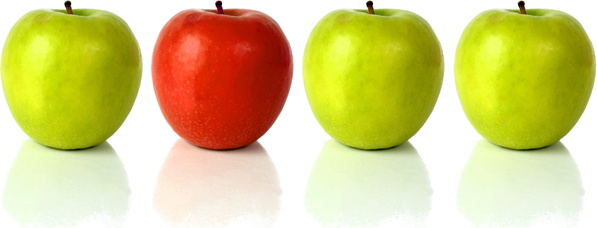
\includegraphics[scale=0.20]{res/images/differenze}
\end{textblock*}

\begin{itemize}
	\item \mbook{} e \mreport{} prevedono i comandi \texttt{chapter}, 
	\texttt{appendix} e \texttt{part} per la segmentazione del documento
	\item \mbook{} permette di gestire la numerazione per frontespizio,
	documento e appendici
	\item \mreport{} e \marticle{} permettono la definizione di un 
	\emph{abstract}
	\item \mbook{} è pensato per documenti con pagine destre e siniste
\end{itemize}

\end{frame}